% !TEX encoding = UTF-8 Unicode

\documentclass[a4paper]{article}

\usepackage{color}
\usepackage{url}
\usepackage[T2A]{fontenc} % enable Cyrillic fonts
\usepackage[utf8]{inputenc} % make weird characters work
\usepackage{graphicx}

\usepackage[english,serbian]{babel}
%\usepackage[english,serbianc]{babel} %ukljuciti babel sa ovim opcijama, umesto gornjim, ukoliko se koristi cirilica

\usepackage[unicode]{hyperref}
\hypersetup{colorlinks,citecolor=green,filecolor=green,linkcolor=blue,urlcolor=blue}

%\newtheorem{primer}{Пример}[section] %ćirilični primer
\newtheorem{primer}{Primer}[section]

\begin{document}

\title{Klimatske promene - mit ili realnost\\ \small{Seminarski rad u okviru kursa\\Tehničko i naučno pisanje\\ Matematički fakultet}}


\author{Ana Šaponjić\\ mi21255@alas.matf.bg.ac.rs \and Elena Zorić\\ mi21300@alas.matf.bg.ac.rs \and Marija Trišović\\ mi21164@alas.matf.bg.ac.rs\and \\Mihajlo Živanović\\ mi21353@alas.matf.bg.ac.rs }
\date{1.~decembar 2022.}


\date{decembar 2022.}
\maketitle
\abstract{
 \footnotesize {
 U ovom tekstu je ukratko objašnjeno šta su  klimatske promene. Kako one utiču na na promene flore  i faune, ali ne samo toga nego i mnogih promena koje mogu dovesti do potpune promene reljefa, takođe koje su posledice svih klimatskih promena i šta one prouzrokuju. Samim tim  ova tema poteže mnogo pitanja. Šta je uzrok, pitanje na koje se daju različiti odgovori.}}

\tableofcontents

\newpage

\section{Uvod}
\label{sec:uvod}
Termin klimatske promene, se do industrijske revolucije je bio vezan za rezultat promena prirodnih okolnosti. Međutim danas termin klimatske promene koristimo kada govorimo o promenama klime od početka dvadesetog veka, koje su nastale kao posledica ljudskih aktivnosti.


Klimatske promene, posebno one koje su u opticaju globalnog zagrevanja, postaju ozbiljnim problemom za prirodu i ljudsko društvo. Njihove posledice su očigledne kada su u pitanju biodiverzitet, biljne i životinjske vrste, pa i čovek. Temperature rastu, i topi led ma polovima, samim tim se nivo mora povećava , što utiče na floru i faunu na priobalnom području zvoj 
Mišljenje stručnjaka je podeljno. Jedni misle da su ove promene samo deo razvoja planete i da je čovekov uticaj jako mali.




\section{Topljenje glečera}
\label{sec:toplenje_glečera}
Globalno zagrevanje će dovoditi do rasta nivoa mora usled topljenja leda, a taj porast nivoa mora može trajati čitav milenijum .Klimatske promene predstavljaju „primarni ekološki izazov“ prvog veka trećeg milenijuma. Istraživanja Grenlanda su pokazala da je glečer 2012. ušao u fazu nestajanja i završavanja leda u vodama severnog Atlantika. Ipak se leti otopi veća količina leda od one koja se ne može nadoknaditi zimi. To dovodi do toga da se manje sunčeve svetlosti odbija od površinu okeana, voda više apsorbuje toplotu i postaje toplija.

Na Antarktiku je primijećena džinovska rupa za koju naučnici tvrde da je rascjep ledene površine veći od teritorije Holandije. Zato uporno ukazuju na moguću kataklizmu – Arktik bez leda do 2040. godine.
Ukoliko bi se to dogodilo, to bi značilo da bi Arktik postao velikim vodenim područjem koje bi promijenilo floru i faunu, biodiverzitet i ekosisteme. Naravno, u takvoj situaciji nestale bi 20 mnoge biljne i životinjske vrste kao što su, na primer, foke i polarni medvedi. Pretpostavlja se da bi, zbog klimatskih promena, u slijedećih nekoliko decenija moglo doći do izumiranja polarnih medveda.

\begin{figure}[!ht]
\begin{center}
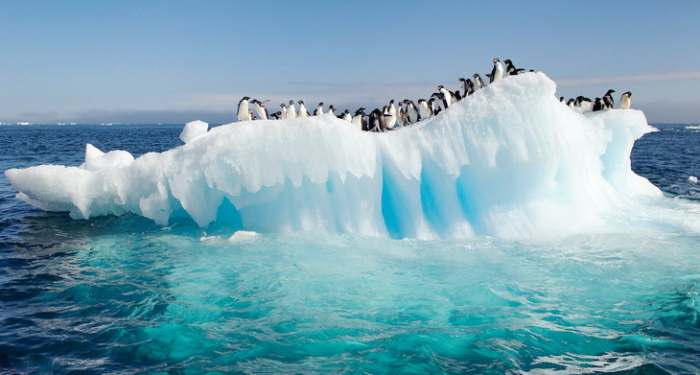
\includegraphics[scale=0.5]{slika2.jpg}
\end{center}
\caption{Topljenje glečera}
\label{fig:glecer}
\end{figure}

\section{Promene klimatskih obrazaca
i elementarne nepogode}	
\label{sec:promene_klimatskih_obrazaca}
Ono što je sada već poznato jeste da suvi regioni postati još suvlji. To znači da u regionima koje imaju malo padavina će biti sve manje, dok će regioni  koji su vlažni iskusiti povećanje padavina. 
Brojnim istraživanjima je dokazano jeste da padavine traju kraće ali da su intenzivije. Na primer umesto da padavina traje nedelju dana umerenim intezitetom, za 2 dana će pasti ista količina padavina. To dovodi do povećanog rizika od poplava.

Naučnici su ipak jasno upozorili da jedan klimatski poremećaj ne može da se pripiše samo ekstremnim posledicama klimatskih promena globalnog zagrevanja dovode do velikih oscilacija u temperaturama. Samo u 2014. godini ih je bilo pogođeno 39,7 miliona, u poplavama 36,6 i u olujama 25,7 miliona. Pod uticajem globalnog zagrevanja, javljaju se velike vrućine čije temperature stvaraju  požare.

Klimatske promene sa svojim promenjenim klimatskim obrascima prouzrokuju izumiranje nekih biljnih i životinjskih vrsta. 

\section{Efekat staklene bašte}	
\label{sec:efekat_staklene_baste}
Efekat staklene bašte je proces zagrevanja Zemlje koji je nastao poremećajem energetske ravnoteže između količine zračenja koje Zemljina površina prima od Sunca i vraća u svemir. Deo toplotnog zračenja, koje stiže do Zemljine kore, odbija se u atmosferu i, umesto da ode u svemir, apsorbuju ga neki gasovi u atmosferi i ponovno dozračuju na Zemlju. Na ovaj način se temperatura Zemljine površine povišava.

\begin{figure}[!ht]
\begin{center}
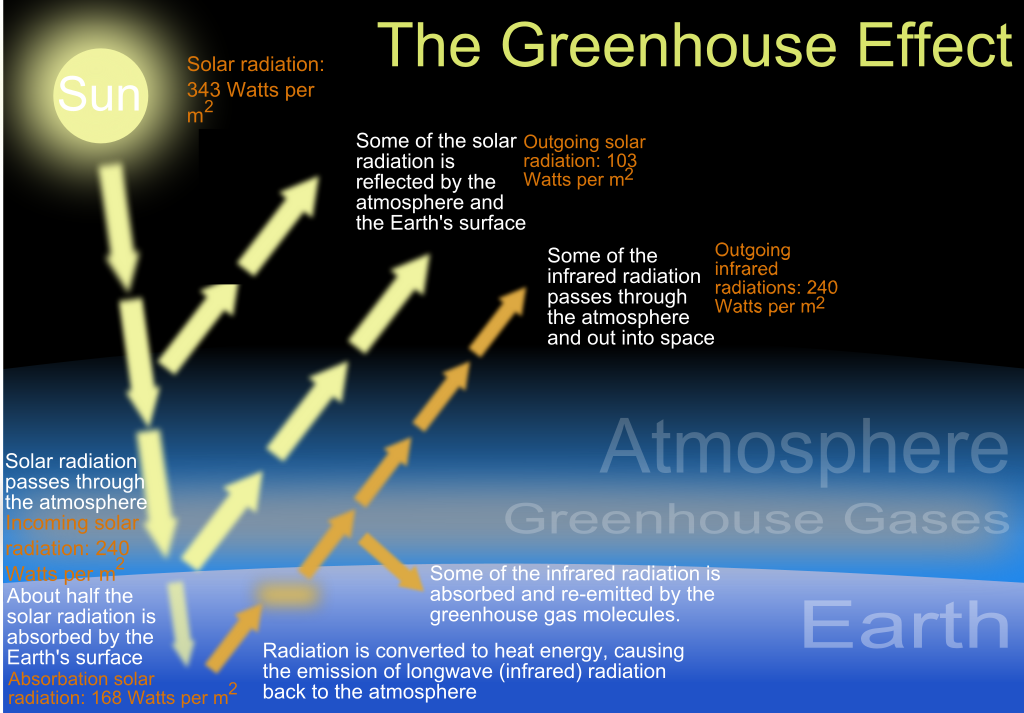
\includegraphics[scale=0.26]{slika3.png}
\end{center}
\caption{Efekat staklene bašte}
\label{fig:efekat}
\end{figure}

\section{Uticaj na biodiverzitet i ekosisteme}
\label{sec:uticaj_na_biodiverzitet_i_ekosisteme}
Opstanak ekosistema zavisi od biodiverziteta, odnosno od biološke raznolikosti biljaka i životinja. Na Zemlji je sve manje životinja, biljaka i pitke vode. Prema četiri naučna izveštaja UN o biodiverzitetu sve to dešava se velikom brzinom. Ako se trenutni trendovi nastave, na američkom kontinentu će do 2050. biti 15 procenata manje životinja nego što ih je sada, u Aziji do 2048. godine više neće biti ribe za komercijalni ribolov, Afrika bi do 2100. mogla da izgubi polovinu nekih vrsta ptica i sisara, a više od četvrtine vrsta koje žive u Evropi bilo bi ugroženo.

„Nekim vrstama preti izumiranje. Drugih je sve manje. Da li ljudi imaju pravo da ih dovedu do izumiranja?“ ističe Robert Votson, predsednik istraživačkog tima.

Juval Noa Harari govori o antropogeno determiniranim „talasima istrebljenja“ ističući da su oni vezani za čovekov način proizvodnje. Tri su do sada značajna talasa istrebljenja – prvi, sa širenjem sakupljačke privrede, drugi sa širenjem poljoprivrede, a treći sa početkom industrijalizacije. Obično se ističe da je gotovo trećina životinjskih vrsta ugrožena usljed lošeg djelovanja ljudi, djelovanja koje za posljedicu ima i antropogeno determinirane klimatske poremećaje.

\begin{center}
\begin{tabular}{||c c||} 
 \hline
 1. & snežni leopard \\ 
 \hline
 2. & beli aligator \\ 
 \hline
 3. & beli lav \\
 \hline
 4. & plavi jastog \\
 \hline
 5. & crvena panda \\ 
 \hline
\end{tabular}
\end{center}

\section{Promene u poljoprivredi i erozija tla}
\label{sec:promene_u_poljoprivredi_i_erozija_tla}
Ekstremni vremenski uslovi ugrožavaju proizvodnju hrane, ona opada, a cene namirnica rastu. Klimatske promene globalnog zagrevanja
su se odrazile i na poljoprivredu i ekosisteme. Prema Izveštaju Ujedinjenih nacija o ljudskom razvoju (UNDP, 1998), trećina svetskog stanovništva izdržava se, manje ili više, direktno od zemlje - od onoga što gaje na njivama i od divljači koju love. Ta je populacija, stoga, naročito osetljiva na promene koje utiču na njihovu sposobnost da žive od zemlje.

U mnogim oblastima Azije i Afrike, u kojima postoji brz priraštaj stanovništva, problem razaranja tla preti da osiromaši milione ljudi. Razaranje tla jeste proces u kojem dolazi do pogoršavanja kvaliteta zemlje, a njeni dragoceni prirodni sastojci sve više nestaju zbog prekomerne upotrebe, suše ili neadekvatnog načina đubrenja. Dugoročni efekti razaranja tla ostavljaju ozbiljne posledice, a sam proces teško može da se zaustavi. U onim područjima u kojima je tlo lošeg kvaliteta, dolazi do opadanja poljoprivredne produktivnosti i sve je manje raspoložive plodne zemlje.
Pustošenje tla odnosi se na primere intenzivnog razaranja tla, što dovodi do pretvaranja većih površina gotovo u pustinje. Kao posledica ove pojave, došlo je do formiranja pustinjskih oblasti koje zahvataju površinu koliko Rusija i Indonezija zajedno, izlažući, na taj način, riziku više od 110 zemalja.

\section{Problemi sa vodom}
\label{sec:problemi_sa_vodom}
Za vodu se sasvim ispravno kaže da je „izvor života“. Prema Svetskoj zdravstvenoj organizacija (WHO), dnevne potrebe za vodom iznose od 50-100 litara. Čista i pitka voda je neophodna za obezbeđenje metabolizma, higijene,  zdravlja i života, kao i za ukupnu dobrobit vezanu za kulturni i civilizacijski razvoj.

Ipak, količina vode za piće je ograničena. Izuzetno velika količina vode se nekontrolisano troši u domaćinstvima, industriji i poljoprivredi što se nepovoljno odražava na zadovoljavanje osnovnih potreba velikog broja stanovništva tako da će ta neokontrolisanost upotrebe vode ugroziti svetsku proizvodnju žitarica i veliki broj ljudi. Samo u poslednjoj polovini veka, utrostručena je upotreba vode.

Jasno je da će povećana upotreba vode, kao i veliki porast stanovništva, klimatske promene, zatim smanjenje količine podzemnih voda, reka i jezera, dovesti do povećane zagađenosti vode i njene nestašice. Voda pripada obnovljivim prirodnim resursima, međutim, narušavanjem ekološke ravnoteže dolazi i do iscrpljivanja i nedostatka resursa pa, prema tome, i vode kao resursa.

Potencijalna i stvarna područja sukoba za vodu i oko vode odnose se na Bliski istok, Tursku, Irak i Siriju, a zatim na područja Egipta, Etiopije i Sudana, Senegala i Mauritanije, Indije, Pakistana i Kine.

\end{document}
